\documentclass[letterpaper,11pt]{article}
\newlength{\outerbordwidth}
%\pagestyle{empty}
\raggedbottom%
\raggedright%
\usepackage{graphicx, wrapfig}
\usepackage{multirow}
\usepackage[svgnames]{xcolor}
\usepackage{framed}
\usepackage{tocloft}
\usepackage{enumerate}

% set font default
\renewcommand*\familydefault{\sfdefault} 	
\usepackage[T1]{fontenc}

% more font size definitions
\usepackage{moresize}		
% \usepackage{fontawesome}
\usepackage{fontawesome5}

%----------------------------------------
\usepackage{geometry}
\pagestyle{empty} %Clean page style, No headers, footers or page numbers
\geometry{letterpaper,tmargin=1in,bmargin=1in,lmargin=1in,rmargin=1in,headheight=0in,headsep=0in,footskip=.3in}

\setlength{\parindent}{0mm} %No identation at the first line of paragraphs
\setlength{\parskip}{0mm} %No distance between paragraphs
\setlength{\itemsep}{0mm} %No space between items
\setlength{\topsep}{0mm} %No distance at the beginning of item lists
\setlength{\tabcolsep}{0mm} %Space in table columns

%----------------------------------------------------------------------------------------
%	Color DEFINITIONS
%---------------------------------------------------------------------------------------- 
\usepackage{transparent}
\usepackage{color}

%accent color
\definecolor{complcol}{RGB}{250,150,10}

%dark background color
\definecolor{bgcol}{RGB}{110,110,110}

%light background / accent color
\definecolor{softcol}{RGB}{225,225,225}

\definecolor{sectcol}{RGB}{0,120,150}

\definecolor{boldgrey}{RGB}{170,170,170}
\definecolor{boldblue}{RGB}{7,45,171}

\definecolor{darkblue}{rgb}{0.0,0.0,0.5}


\definecolor{shadecolor}{gray}{1}  % Outer background color of title bars (0 = black, 1 = white)
\definecolor{shadecolorB}{gray}{0.9}  % Inner background color of title bars
%-----------------------------------------------------------
\setlength{\outerbordwidth}{0.93pt}  % Width of border outside of title bars

%-----------------------------------------------------------
%Margin setup

\setlength{\evensidemargin}{-0.25in}
\setlength{\headheight}{0in}
\setlength{\headsep}{0in}
\setlength{\oddsidemargin}{-0.25in}
\setlength{\paperheight}{11in}
\setlength{\paperwidth}{8.5in}
\setlength{\tabcolsep}{0in}
\setlength{\textheight}{9.5in}
\setlength{\textwidth}{7in}
\setlength{\topmargin}{-0.3in}
\setlength{\topskip}{0in}
\setlength{\voffset}{0.1in}

%----------------------------------------------------------
%header and footer
\usepackage{fancyhdr}
\usepackage{lastpage}
\pagestyle{fancy}
\lhead{}
\chead{}
\rhead{}
\lfoot{}
\cfoot{\textit{R.J.Ferreira, Curriculum Vitae, p.~\thepage~of~\pageref{LastPage}}}
\rfoot{}
\renewcommand{\headrulewidth}{0pt}
\renewcommand{\headrulewidth}{0pt}

%----------------------------------------------------------
\usepackage[colorlinks = true,
            linkcolor=black,
            urlcolor=black,
            citecolor=black,
            anchorcolor=black]{hyperref}

% Allow different colors for links in the same document
\newcommand{\customHref}[1]{
    \hypersetup{urlcolor=#1}
}



%-----------------------------------------------------------
%Custom commands

\newcommand{\resitem}[1]{\item #1 \vspace{2pt}}

\newcommand{\resheading}[1]{\vspace{4pt}
  \parbox{\textwidth}{\setlength{\FrameSep}{\outerbordwidth}
    \begin{shaded}
\setlength{\fboxsep}{0pt}\framebox[\textwidth][l]{\setlength{\fboxsep}{4pt}\fcolorbox{shadecolorB}{shadecolorB}{\textbf{\sffamily{\mbox{~}\makebox[6.762in][l]{\large #1} \vphantom{p\^{E}}}}}}
    \end{shaded}
  }\vspace{4pt}
}

\newcommand{\cvevent}[1]{\vspace{5pt}
  \parbox{\textwidth}{\setlength{\FrameSep}{\outerbordwidth}
    \begin{shaded}
        \setlength{\fboxsep}{0pt}{\setlength{\fboxsep}{4pt}\fcolorbox{sectcol}{sectcol}{\textbf{\sffamily{\mbox{~}\makebox[6.762in][l]{\textcolor{white}{\large \uppercase{#1}}} \vphantom{p\^{E}}}}}}
    \end{shaded}
  }\vspace{40pt}
}

% \newcommand{\ressubheading}[4]{
% \begin{tabular*}{6.5in}{l@{\cftdotfill{\cftsecdotsep}\extracolsep{\fill}}r}
% 		\textbf{#1} & #2 \\
% 		\textit{#3} & \textit{#4} \\
% \end{tabular*}\vspace{-6pt}}

\newcommand{\ressubheading}[4]
{
    \begin{tabular*}{6.5in}{@{\extracolsep{\fill}}l r}
        {\textbf{#1}}&{\textbf{#2}}\\
        {\textit{#3}}&{#4}
    \end{tabular*}
}

\newcommand{\bigheader}[1]{
	\begin{center}
		\fontfamily{phy}
		\selectfont\Huge\scshape#1
	\end{center}
}

\newcommand{\longline}{
	\vspace{-8pt} \rule{\textwidth}{1pt}
	\vspace{8 pt}
}


\newcommand{\icon}[3]{\makebox(#2, #2){\textcolor{#3}{\csname fa#1\endcsname}}}	%icon shortcut
\newcommand{\icontext}[4]{ 						%icon with text shortcut
	\vcenteredhbox{\icon{#1}{#2}{#4}} \vcenteredhbox{\textcolor{#4}{#3}}
}

\providecommand*\email[1]{\href{mailto:#1}{#1}}

\newcommand{\name}{Ricardo Jorge de Ara\'ujo Ferreira}
\newcommand{\birth}{January 19, 1985}
\newcommand{\faddress}{Rua Conde de Ferreira 97, 4$^{\circ}$D }
\newcommand{\saddress}{4580 - 407 Paredes} %chktex 8
\newcommand{\taddress}{Paredes, Portugal}
\newcommand{\mobilephone}{\faMobile*\hspace{3pt}+351 91 615 15 65}
\newcommand{\princemail}{\faPaperPlane\hspace{3pt}\customHref{black}\href{mailto:ricarraf@gmail.com}{ricarraf@gmail.com}}
\newcommand{\github}{\faGithub\hspace{3pt}{\href{https://www.github.com/ricardojaferreira}{/ricardojaferreira}}}
\newcommand{\linkedin}{\faLinkedin\hspace{3pt}\href{https://www.linkedin.com/in/RicardoAraujoFerreira}{/RicardoAraujoFerreira}}

%-----------------------------------------------------------


\begin{document}
%\thispagestyle{empty} % this page has no header  

\bigheader{Curriculum Vitae}
\longline%

%%%%%%%%%%%%%%%%%%%%%%%%%%%%%%
% \cvevent{\faDatabase\hspace{4pt}Biodata}
\resheading{\faAddressCard\hspace{4pt}Biodata}
%%%%%%%%%%%%%%%%%%%%%%%%%%%%%%


\begin{tabular*} {6.9in}{ll@{\extracolsep{\fill}}r}
\multirow{9}{*}{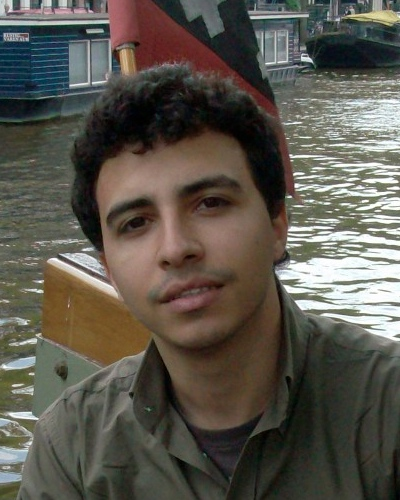
\includegraphics[scale=0.25]{img/picture.jpg}} & \hspace{0.2in} \textbf{\Large \name} & \textbf{\birth}\\
 & \hspace{0.2in} Electrical and Computer Science Engineer (M.Sc.) 	& 			 \\
  & \hspace{0.2in} {\footnotesize Student of Master in Informatics and Computing Engineering\par} 	& 			 \\

 &									& 			\\
 & \hspace{0.2in} \faddress& \princemail\\
 & \hspace{0.2in} \saddress& \github\\
 & \hspace{0.2in} \taddress& \linkedin		\\ %chktex 1
 &		&		\\
 & \hspace{0.2in}\mobilephone& \\
 &	 	&		\\
\end{tabular*}

\vspace{0.2in}		%%%%%%ATENTION SPACE%%%%


%%%%%%%%%%%%%%%%%%%%%%%%%%%%%%
% \cvevent{\faUser\hspace{4pt}Summary}
\resheading{\faUser\hspace{4pt}Summary}
%%%%%%%%%%%%%%%%%%%%%%%%%%%%%%
\begin{center}
	\parbox{6.762in}{I obtained my master degree in Electrical and Computer science Engineering at the Faculdade de Engenharia da Universidade do Porto, Portugal in 2008. My master thesis was in the field of Power electronics, control drives and measurement techniques, resulting in a group of power converters to be used in a solar Electric Car. %chktex 1
	
	Since then I have been trying to acquire experience and pursuing challenging job opportunities. For 3,5 years I have worked at Efacec, SA, as a control/automation engineer. At first my main activity was the development of automation and telecontrol solutions for electric power systems. When I acquired more experience I have started training new employees and to manage engineering projects, coordinate teams, allocate resources, supervising and find ways to improve processes and reduce the developing time.
	
	When a new opportunity arose at the Institute for Systems and Computer Science of Porto to integrate the renewable energies team I took it. At this job, as a researcher in the field of power converters for electric vehicles and intelligent power grids, I have increased my technical and planning skills. I had also the opportunity to write scientific papers and to present them on international conferences. Being an R\&D engineer was a great opportunity to go out of my comfort zone and to test new and challenging areas. During this job I found out that I really love to develop software.
	
	I started to develop some tiny softwares to help on my everyday tasks, applications running on the web and locally, that perform data analysis, file creation and manipulation, integration with databases and others. And some applications just to learn and have fun.
	
	Sometime later, I started to work has a developer and I am working on that area since then. I am currently working has a full stack developer in an Agile (scrum) environment with technologies like, Javascript, PHP, MySql, Java, Apache Servers, AWS, Git, integration with APIs, and others.
	
	To learn more about software development, algorithms and new programming languages, I have started the \textbf{Master Degree in Informatics and Computing Engineering} at Faculdade de Engenharia, I am currently at the 4rd year out of a 5 year program. }
\end{center}

\vspace{0.8in}		%%%%%%ATENTION SPACE%%%%
\newpage

%%%%%%%%%%%%%%%%%%%%%%%%%%%%%%
\resheading{\faBriefcase\hspace{4pt}Work Experience}
%%%%%%%%%%%%%%%%%%%%%%%%%%%%%%
\begin{itemize}
\item 
	\ressubheading{Web Engineer - Fullstack Developer}{Feb 2018 - Present}{Jumia - Porto Tech Center}{Porto, Portugal} %chktex 8
	\begin{itemize}
		\resitem{Development of software solutions using JAVA frameworks, Spring and Play;}
        \resitem{Database managament and design, (Postgres and Mysql);}
		\resitem{Technical Specification and development of business requirements and improvements;}
		\resitem{Integration with third party software and tools;}
        \resitem{Development of solutions with a strong concern about clean code and architecture;}
        \resitem{Working in an environment with the DevOps culture;}
	\end{itemize}
\item 
	\ressubheading{Fullstack Developer}{May 2014 - Feb 2018}{Gravity Demand, Lda (E-Commerce)}{Penafiel, Portugal} %chktex 8
	\begin{itemize}
		\resitem{Development and integration of software solutions, client/sever programming (JAVA, PHP, Javascript, SQL, CSS, HTML5);}
		\resitem{User interface and usability development and improvement;}
		\resitem{Integration with external services (REST and other API's);}
		\resitem{Technical specification, design and architecture;}
		\resitem{Management of the e-commerce platform;}
		\resitem{Management and coordination between work teams (Marketing, Design, Sales, Development).}
	\end{itemize}
\item
	\ressubheading{R\&D Engineer}{Jan. 2012 - May. 2014}{INESC, Institute for Systems and Computer Engineering}{Porto, Portugal}%chktex 8
	\begin{itemize}
		\resitem{Research, testing and development of power converters for electric vehicles and power grids;}
        \resitem{Design of analog and digital feedback control systems (Software and hardware);}
		\resitem{Validate emerging concepts in Smart-Grids and Renewable Energy systems  by developing electronic prototypes;}
		\resitem{Coordination and planning of the activities and resources for the development laboratories;}
        \resitem{Development of software for validating concepts and make complex computations (C++ and JAVA).}
	\end{itemize}

\item 
	\ressubheading{Control and Automation Engineer, Junior manager}{Aug. 2008 - Jan. 2012}{Efacec, Sistemas de Engenharia SA}{Maia, Portugal} %chktex 8
	\begin{itemize}
		\resitem{Development of control and automation architectures for the Portuguese electric power system (Distribution and Transport Substations - 15kW to 400kW);} %chktex 8
		\resitem{Commissioning and development of factory and site acceptance tests for electric power systems;}
		\resitem{Management and configuration of large IP based Networks and information systems based on UNIX platforms;}
		\resitem{Management of engineering projects (Planning Schedules and coordinate activities).}
	\end{itemize}
\item
	\ressubheading{FEUP Project}{FEUP, Porto}{Undergraduate Teaching Assistant}{Sept. 2007 - Jan. 2008}%chktex 8
	\begin{itemize}
		\resitem{Teach how to organize and develop an engineering project.}
		\resitem{Led weekly course seminars.}
	\end{itemize}
\end{itemize}



%%%%%%%%%%%%%%%%%%%%%%%%%%%%%%%%%%%%%%%%%%%%%%%%
\resheading{\faGraduationCap\hspace{4pt}Education}
%%%%%%%%%%%%%%%%%%%%%%%%%%%%%%%%%%%%%%%%%%%%%%%%
\begin{itemize}
\item
	\ressubheading{MsC in Informatics and Computation Engineering}{Present}{Faculdade de Engenharia da Universidade do Porto}{Porto, Portugal}
	\begin{itemize}
		\resitem{Currently at the 4rd Year, 2 more to finish the graduation.}
		\resitem{\bf Principal Subjects so far: }
			\begin{itemize}
				\resitem{Languages and Web Technologies; Computation Theory; Algorithms; Discreet Mathematics, Oriented Programming Languages, Operating Systems, Databases, Software Engineering, Formal tests in software}
			\end{itemize}
	\end{itemize}
\vspace{2pt}
\item
	\ressubheading{MsC in Electrical and Computers Engineering}{2008}{Faculdade de Engenharia da Universidade do Porto}{Porto, Portugal}%chktex 8
    \begin{itemize}
		\resitem{{\bf Major: }Automation and Control Systems}
		\resitem{{\bf Specialization: }Power and Industrial Electronics and Instrumentation}
		\resitem{{\bf Thesis: }Solar Car. (Classified with 17 out of 20)}
    \end{itemize}
\end{itemize}
%%\vspace{0.1in}		%%%%%%ATENTION SPACE%%%%

%%%%%%%%%%%%%%%%%%%%%%%%%%%%%%
\resheading{\faComment\hspace{4pt}Languages}
%%%%%%%%%%%%%%%%%%%%%%%%%%%%%%

\begin{tabular} {l c l}

	\multicolumn{3}{l}{\hspace{0.05in} (Scale: 1 - Basic, 5 - Very Good)} \\%chktex 8
\\
	\hspace{0.1in} {\bf Portuguese}		& \hspace{0.8in} 5	& \hspace{0.3in} (Mother Tongue)					\\
	\hspace{0.1in} {\bf Italian}			& \hspace{0.8in} 5	& \hspace{0.3in} (My Father is Italian)				\\
	\hspace{0.1in} {\bf English}		& \hspace{0.8in} 5	& \hspace{0.3in} (Obtained the international C1 Level)	\\
	\hspace{0.1in} {\bf Spanish}		& \hspace{0.8in} 3	& \hspace{0.3in}								\\

\end{tabular}

%%%%%%%%%%%%%%%%%%%%%%%%%%%%%%
\resheading{\faCertificate\hspace{4pt}Skills}
%%%%%%%%%%%%%%%%%%%%%%%%%%%%%%

\begin{itemize}
\item
	Programming and Markup Languages
	\begin{itemize}
		\resitem{{\bf Expert:}  JAVA, CSS, HTML5, JSON, SQL, PHP, JavaScript, C/C++, \LaTeX}
		\resitem{{\bf Intermediate:} Python, Scala, XML }
    \end{itemize}
\end{itemize} 
\hspace{20pt}
\begin{itemize}
\item
	Frameworks
	\begin{itemize}
		\resitem{{\bf Expert:} Spring, Laravel, Bootstrap, LESS}
		\resitem{{\bf Intermediate:} Play, Zend, ReactJs}
	\end{itemize}
	
	\item
	Test and Debug
	\begin{itemize}
		\resitem{Junit, PHPunit, Xdebug, Cucumber, Gherkin}
	\end{itemize}

\item
	Tools and Software
	\begin{itemize}
		\resitem{{\bf Expert:} UNIX Shell, Docker, MongoDb, ElasticSearch, Prometheus, Grafana, MySQL/MariaDb, Apache 2, Magento, GIT, Jenkins}
		\resitem{{\bf Intermediate:} PostgreSQL, Couchbase, RabbitMQ, Nginx, Hazelcast, Memcached}
	\end{itemize}
	
	\item
	Operating Systems
	\begin{itemize}
		\resitem{Mac OS X, Linux, Microsoft Windows}
	\end{itemize}

	\item
	Social
	\begin{itemize}
		\resitem{People person, enjoys being challenged, hardworking, leadership, entrepreneurial, organized.}
	\end{itemize}
\end{itemize}

%\vspace{0.8in}		%%%%%%ATENTION SPACE%%%%

%%\newpage

\vspace{5mm}

\begin{figure}[h]
\centering
{
\includegraphics[scale=0.25]{img/sig.png}}
\end{figure}

\end{document}
